\documentclass[aspectratio=43]{beamer}
\usepackage[english]{babel}
\usepackage{graphicx}
\usepackage{amsthm}
\usepackage{mathtools}
\usepackage{physics}
\usepackage{calligra}
\usepackage{csquotes}
\usepackage{tensor}
\usepackage[thicklines]{cancel}
\usepackage{tcolorbox}
\usepackage{pstricks}
\usepackage[backend=biber, bibstyle=nature, sorting=nty, citestyle=numeric-comp]{biblatex} %Custom bibliography
    \addbibresource{bib.bib} %Load references


\DeclareMathAlphabet{\mathcalligra}{T1}{calligra}{m}{n}
\DeclareFontShape{T1}{calligra}{m}{n}{<->s*[2.2]callig15}{}
\newcommand{\scriptr}{\mathcalligra{r}\,}
\newcommand{\boldscriptr}{\pmb{\mathcalligra{r}}\,}
\def\rc{\scriptr}
\def\brc{\boldscriptr}
\def\hrc{\hat\brc}
\newcommand{\ie}{\emph{i.e.}} %id est
\newcommand{\eg}{\emph{e.g.}} %exempli gratia
\newcommand{\rtd}[1]{\ensuremath{\left\lfloor #1 \right\rfloor}}
\newcommand{\dirac}[1]{\ensuremath{\delta \left( #1 \right)}}
\newcommand{\diract}[1]{\ensuremath{\delta^3 \left( #1 \right)}}
\newcommand{\e}{\ensuremath{\epsilon_0}}
\newcommand{\m}{\ensuremath{\mu_0}}
\newcommand{\V}{\ensuremath{\mathcal{V}}}
\newcommand{\prnt}[1]{\ensuremath{\left(#1\right)}} %parentheses
\newcommand{\colch}[1]{\ensuremath{\left[#1\right]}} %square brackets
\newcommand{\chave}[1]{\ensuremath{\left\{#1\right\}}}  %curly brackets

\useoutertheme{infolines}
\useinnertheme{rectangles}
\usefonttheme{professionalfonts}


\definecolor{orange}{HTML}{69B46F}
\definecolor{gray}{HTML}{303030}
\definecolor{yellow}{HTML}{f0be52}
\definecolor{lightorange}{HTML}{f19e58}

\renewcommand{\CancelColor}{\color{orange}}

\makeatletter
\newcommand{\mybox}[1]{%
  \setbox0=\hbox{#1}%
  \setlength{\@tempdima}{\dimexpr\wd0+13pt}%
  \begin{tcolorbox}[colback=orange,colframe=orange,boxrule=0.5pt,arc=4pt,
      left=6pt,right=6pt,top=6pt,bottom=6pt,boxsep=0pt,width=\@tempdima]
    \textcolor{white}{#1}
  \end{tcolorbox}
}
\makeatother

\usecolortheme[named=orange]{structure}
\usecolortheme{sidebartab}
\usecolortheme{orchid}
\usecolortheme{whale}
\setbeamercolor{alerted text}{fg=yellow}
\setbeamercolor{block title alerted}{bg=alerted text.fg!90!black}
\setbeamercolor{block title example}{bg=lightorange!60!black}
\setbeamercolor{background canvas}{bg=gray}
\setbeamercolor{normal text}{bg=gray,fg=white}

\setbeamertemplate{footline}
        {
      \leavevmode%
      \hbox{%
      \begin{beamercolorbox}[wd=.333333\paperwidth,ht=2.25ex,dp=1ex,center]{author in head/foot}%
        \usebeamerfont{author in head/foot}\insertshortauthor~~(\insertshortinstitute)
      \end{beamercolorbox}%
      \begin{beamercolorbox}[wd=.333333\paperwidth,ht=2.25ex,dp=1ex,center]{title in head/foot}%
        \usebeamerfont{title in head/foot}\insertshorttitle
      \end{beamercolorbox}%
      \begin{beamercolorbox}[wd=.333333\paperwidth,ht=2.25ex,dp=1ex,center]{date in head/foot}%
        \usebeamerfont{date in head/foot}\insertshortdate{}%\hspace*{2em}

    %#turning the next line into a comment, erases the frame numbers
        %\insertframenumber{} / \inserttotalframenumber\hspace*{2ex} 

      \end{beamercolorbox}}%
      \vskip0pt%
    }


\setbeamertemplate{blocks}[rectangle]
\setbeamercovered{dynamic}

\setbeamertemplate{section page}
{
	\begin{centering}
		\begin{beamercolorbox}[sep=27pt,center]{part title}
			\usebeamerfont{section title}\insertsection\par
			\usebeamerfont{subsection title}\insertsubsection\par
		\end{beamercolorbox}
	\end{centering}
}

%\setbeamertemplate{subsection page}
%{
%	\begin{centering}
%		\begin{beamercolorbox}[sep=12pt,center]{part title}
%			\usebeamerfont{subsection title}\insertsubsection\par
%		\end{beamercolorbox}
%	\end{centering}
%}

\newcommand{\hlight}[1]{\colorbox{violet!50}{#1}}
\newcommand{\hlighta}[1]{\colorbox{red!50}{#1}}
\title{Practical Chaos} %->->->->-> Check hyperref title <-<-<-<-<-
\subtitle{Using Dynamical Systems to Encrypt Audio and Visual Data}
\author[J. Ruiter]{Julia Ruiter}
\institute[Capstone Presentation]{
    Scripps College%
    \\%
    Department of Mathematics and Physics%
} %You can change the Institution if you are from somewhere else
\date{May 8, 2019}
%\logo{\includegraphics[width= 0.2\textwidth]{images/a-logo.png}}

\begin{document}
    
    \frame{\titlepage}
    
    \begin{frame}{Summary}
        \tableofcontents
    \end{frame}
    
    \section{What is Chaos?}

    \frame{\sectionpage}
    
    % \begin{frame}{The Butterfly Effect}
    %     \begin{tabular}{p{3cm}c}
    %     \begin{figure}
    %         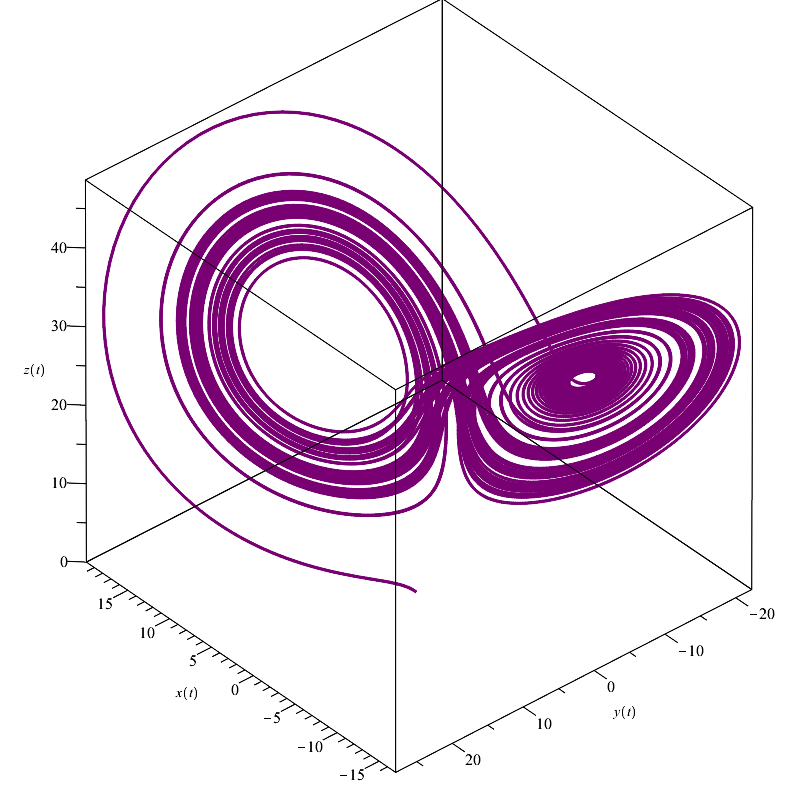
\includegraphics[width=\linewidth]{lorenz2.PNG}
    %     \end{figure}
    %     &
    %     \begin{equation}
    %         \begin{cases} 
    %         \dot{x} = \sigma(y-x) \\ 
    %         \dot{y} = rx - y - xz \\ 
    %         \dot{z} = xy - bz
    %         \end{cases}
    %     \end{equation}  
    %     \end{tabular}
    % \end{frame}       
    \begin{frame}{The Butterfly Effect}
        \begin{figure}
            \centering
            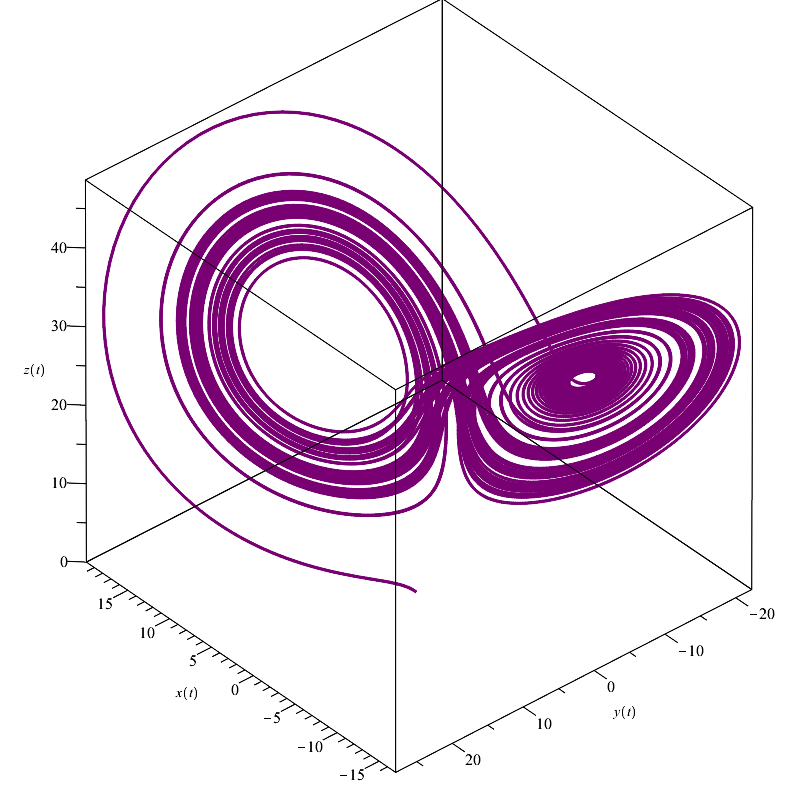
\includegraphics[height=7cm]{lorenz2.PNG}
        \end{figure}
    \end{frame}
    
    \begin{frame}{The Butterfly Effect}
        \begin{equation*}
            \centering
            \begin{cases} 
            \dot{x} = \sigma(y-x) \\ 
            \dot{y} = rx - y - xz \\ 
            \dot{z} = xy - bz
            \end{cases}
        \end{equation*} 
    \end{frame}
    
    \begin{frame}{The Butterfly Effect}
        \begin{figure}
            \centering
            \begin{figure}[ht]
                \begin{minipage}[b]{0.45\linewidth}
                    \centering
                    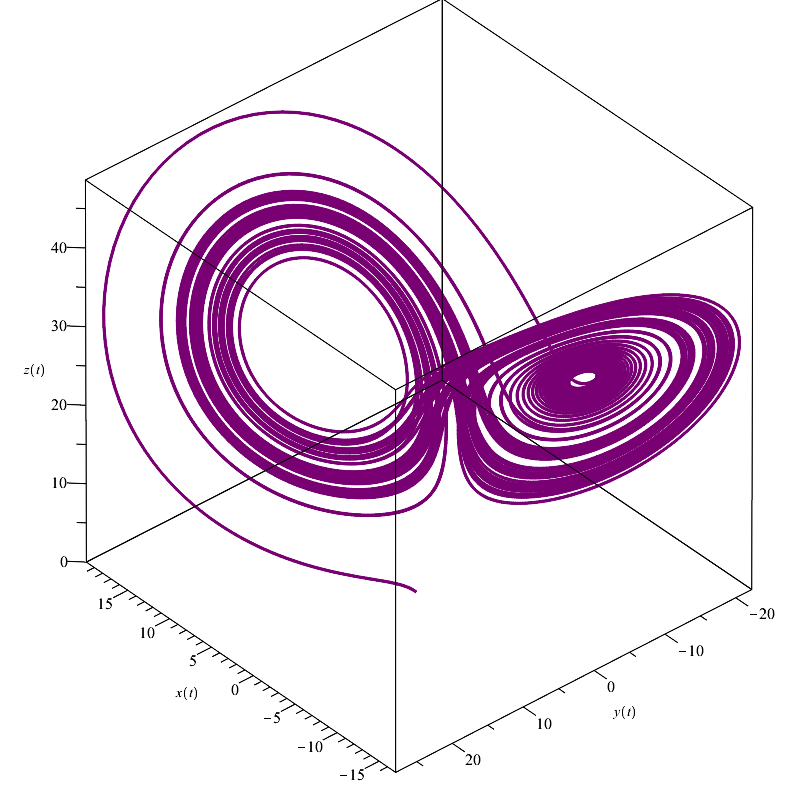
\includegraphics[width=\textwidth, height=5cm]{lorenz22.PNG}
                    \caption{chaotic, $\sigma$ = 10}
                    \label{fig:a}
                \end{minipage}
                \hspace{0.5cm}
                \begin{minipage}[b]{0.45\linewidth}
                    \centering
                    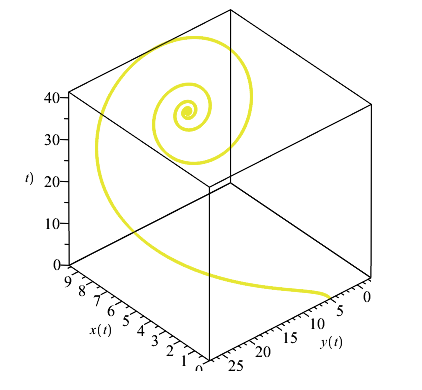
\includegraphics[width=\textwidth, height=5cm]{lorenz_s1.PNG}
                    \caption{non-chaotic, $\sigma$ = 1}
                    \label{fig:b}
                \end{minipage}
            \end{figure}
            % 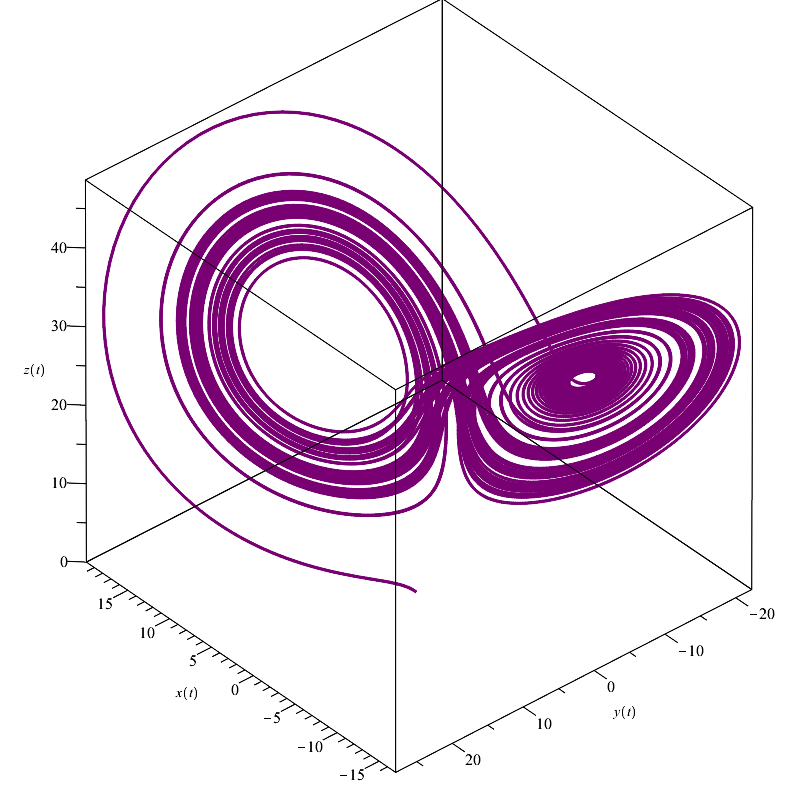
\includegraphics[width=0.6\textwidth]{lorenz2.png}%
            % 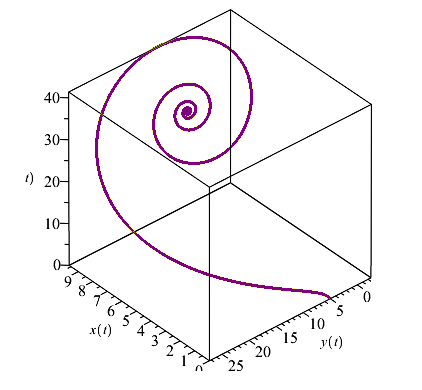
\includegraphics[width=0.4\textwidth]{lorenz_s2.png}
        \end{figure}
    \end{frame}    
    
 
 

    \section{What is Encryption?}
    
    \frame{\sectionpage}
    
    \begin{frame}{Creating a Cryptosystem}
        \centering
        What you need:
        \begin{itemize}
        	\item A message  $m$
        	\item A method to encode  $f$
        	\item A method to decode  $h$
        	\item A key  $k$
        \end{itemize}
    \end{frame}    
      
    \begin{frame}{Creating a Cryptosystem}
        \centering
        \begin{equation*}
            c = f ( m , k )
        \end{equation*}%
        \begin{equation*}
            m = h ( c )
        \end{equation*}%
        \begin{equation*}
            c \neq m   
        \end{equation*}
    \end{frame}
    
    \begin{frame}{Creating a Cryptosystem}
        \begin{minipage}[b]{0.45\linewidth}
            What you need:
            \begin{itemize}
            	\item A message  $m$
            	\item A method to encode  $f$
            	\item A method to decode  $h$
            	\item A key  $k$
            \end{itemize}
        \end{minipage}
        \hspace{0.5cm}
        \begin{minipage}[b]{0.45\linewidth}
            \centering
            \begin{equation*}
                \centering
                \begin{cases} 
                \dot{x} = \sigma(y-x) \\ 
                \dot{y} = rx - y - xz \\ 
                \dot{z} = xy - bz
                \end{cases}
            \end{equation*} 
        \end{minipage}
    \end{frame}
    \section{Chaotic Encryption:  Digital Images}
    
    \frame{\sectionpage}
    
    \begin{frame}{Process}
        \centering
        What to encrypt:
        \begin{itemize}
        	\item Pixel color values (RBG/BW)
        	\item Pixel locations
        \end{itemize}
    \end{frame}    

    % \begin{frame}{Why?}
    %     \begin{figure}
    %         \centering
    %         \includegraphics[height=7cm]{celty.png}
    %     \end{figure}
    % \end{frame}    

    \begin{frame}{How:}
        \centering
        Shuffling Pixel Values, mod 256:
        \begin{equation*}
            f ( p ) := p_{i+1} = \lambda_{1} * p_{i} ( 1 - p_{i} )
        \end{equation*}
        Shuffling pixel locations, mod (image size)
        \begin{equation*}
            g ( p ) := p_{i+1} = \lambda_{2} * p_{i} ( 1 - p_{i} )
        \end{equation*}
    \end{frame}

    \section{Chaotic Encryption:  Sound Bytes}
    
    \frame{\sectionpage}
    
    \begin{frame}
        \centering
        What if you could encrypt real-time?
    \end{frame}
    
    \begin{frame}{Creating a Physical Key}
        \centering
        Components:
        \begin{itemize}
        	\item A message:  $a$ $sound$ $byte$
        	\item A method to encode:  $masking$ $with$ $static$
        	\item A method to decode:  $filtering$ $out$ $static$
        	\item A key:  $coupled$ $systems$
        \end{itemize}
    \end{frame}     
    
    \begin{frame}{The Theory of Coupled Systems}
        \begin{minipage}[b]{0.45\linewidth}
            \centering
            \caption{Master System}
            \label{lst}
            \begin{equation*}
                \begin{cases} 
                    \dot{x_{m}} = \sigma(y-x) \\ 
                    \dot{y_{m}} = rx - y - xz \\ 
                    \dot{z_{m}} = xy - bz
                \end{cases}
            \end{equation*}
        \end{minipage}
        \hspace{0.5cm}
        \begin{minipage}[b]{0.45\linewidth}
            \centering
            \caption{Receiver System}
            \label{lst}
            \begin{equation*}
                \begin{cases} 
                    \dot{y_{r}} = rx - y_{r} - xz_{r} \\ 
                    \dot{z_{r}} = xy_{r} - bz_{r}
                \end{cases}
            \end{equation*}
        \end{minipage}
    \end{frame}
    
    \begin{frame}{A Physical Coupled System}
        \begin{figure}
            \centering
            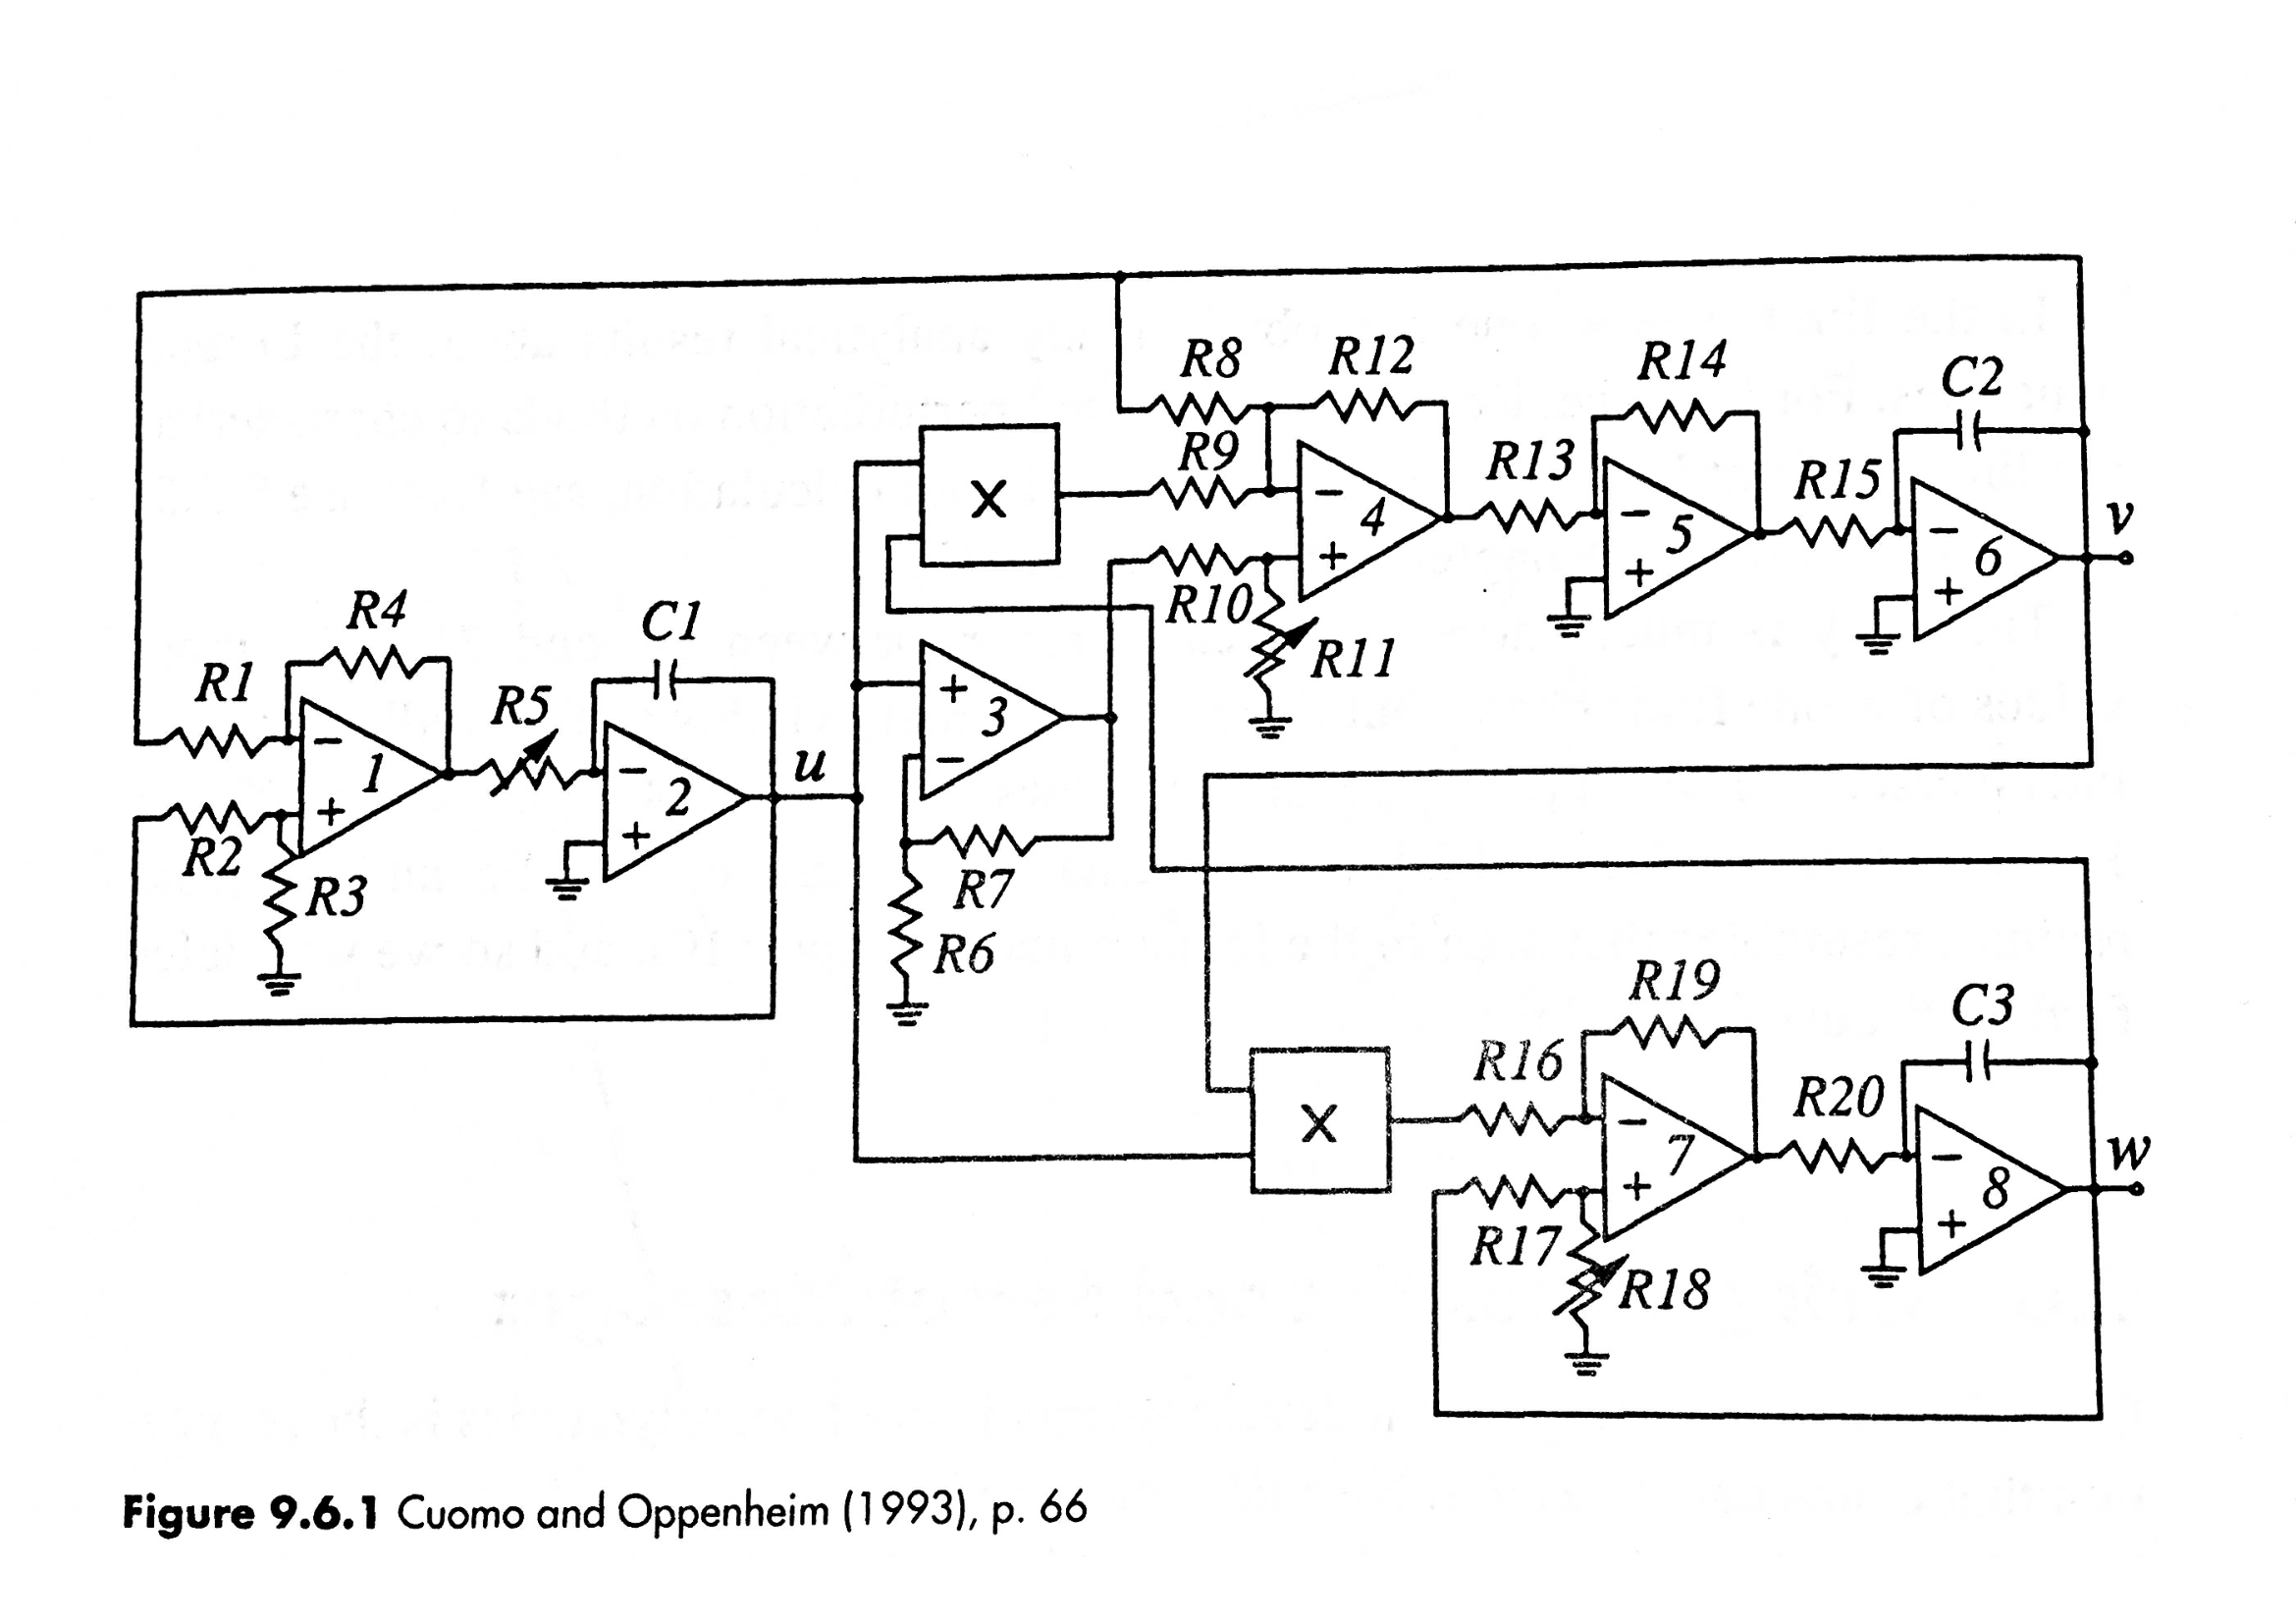
\includegraphics[height=5cm]{circuit.png}
            \caption{this RC circuit is one half of a coupled system}
            \label{fig}
        \end{figure}
    \end{frame}



    
    % \section*{Acknowledgments} %You can remove this if you do not want to use it
    %     \begin{frame}{Acknowledgments}
    %         The author is extremely thankful to Prof. Antônio F. R. T. Piza for the short, yet wonderful, conversations about this seminar.
    %     \end{frame}
    
    \section*{References}%You can remove this if you do not want to use it
        \nocite{Strogatz} \nocite{Koblitz} \nocite{article} \nocite{PhysRevLett.64.821} \nocite{PhysRevLett.71.65} \nocite{MR1917690}  \nocite{MR1604666} \nocite{lorenz1963} \nocite{Nishi} \nocite{Cruz}
        \begin{frame}[allowframebreaks]{References}
            \printbibliography
        \end{frame}

    \section*{Thank you for listening}
    \begin{frame}{}
        \centering
            \Huge\bfseries
        \textcolor{orange}{Questions?}
    \end{frame}
\end{document}
